\documentclass[12pt,a4paper]{article}
\usepackage[utf8]{inputenc}
\usepackage[margin=2cm]{geometry}
\usepackage{amsmath}
\usepackage{amssymb}
\usepackage{amsthm} 
\usepackage{graphicx}
\usepackage{mathtools}

\DeclarePairedDelimiter{\abs}{\lvert}{\rvert}
\newcommand{\inter}{\begin{matrix}\prod\end{matrix}}

\newcommand{\verteq}{\rotatebox{90}{$\,=$}}
\newcommand{\equalto}[2]{\underset{\scriptstyle\overset{\mkern4mu\verteq}{#2}}{#1}}

\renewcommand{\qedsymbol}{\rule{0.7em}{0.7em}}
\usepackage[normalem]{ulem}
\begin{document}

\section{Lezione 15 - Approssimazione polinomiale ai minimi quadrati}
In questa lezione introdurremo un metodo molto importante per l'approssimazione (polinomiale) di una funzione a partire da un campionamento discreto: la cosiddetta approssimazione ai \uline{MINIMI} \uline{QUADRATI} (in inglese \uline{Least Squares} (LS) approximation). Si tratta di una tecnica diversa\\ dall'interpolazione, che ha forti connessioni con la statistica nel
campo dei ``metodi di \uline{regressione}" (di cui non potremo occuparci in questo corso).\\
Per capirne l'interesse applicativo, possiamo fare un paio di esempi.\\
Nel primo, consideriamo il grafico dell'andamento del prezzo di un'azione sul mercato azionario, campionato ogni giorno (ad esempio alla chiusura delle contrattazioni) su un arco temporale esteso (tipo un anno)
\begin{center}
    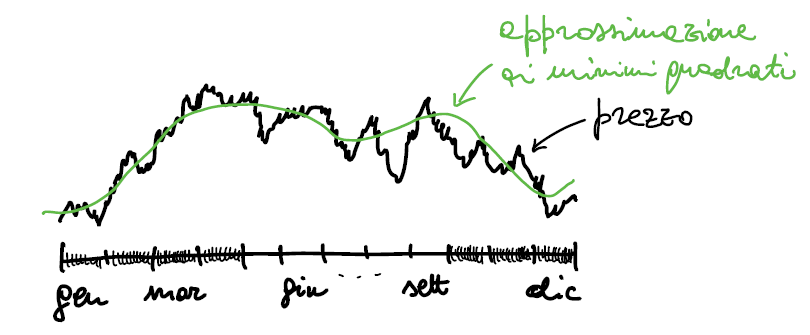
\includegraphics[scale=0.7]{pag2.png}
\end{center}
Si tratta di un fenomeno per sua natura fortemente irregolare (per comodità grafica i valori discreti sono interpolati ad es. linearmente a tratti).\\
Qui una richiesta tipica potrebbe essere quella di REGOLARIZZARE il grafico, cercando una qualche forma di ``medie" dei dati, in modo da evidenziare il trend durante il periodo.
\newline\newline
Nel secondo esempio consideriamo invece un segnale regolare campionato
\begin{center}
    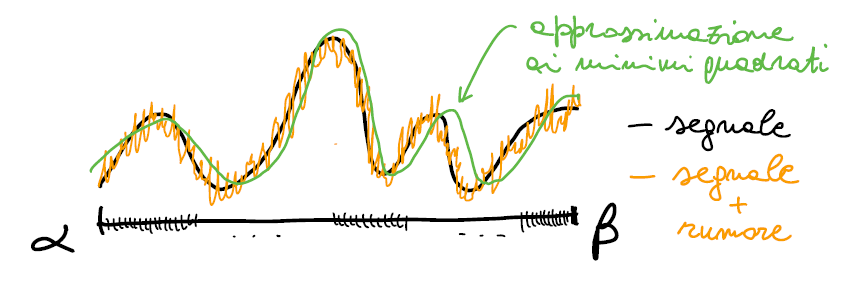
\includegraphics[scale=0.7]{pag3.png}
\end{center}
in presenza di RUMORE (ad es. un segnale audio) con un passo molto piccolo: quello che viene misurato non è il segnale $s$, ma un segnale ``perturbato" $\Tilde{s} = s+r$, dove $r$ è il rumore che si può pensare come una variabile che ``oscilla" ad alta frequenza.\\
Qui una richiesta tipica potrebbe essere quella di FILTRARE il rumore, di nuovo facendo una qualche ``media" dei dati misurati.\\
Se ad esempio volessimo avere un'approssimazione ragionevole della velocità di variazione di $s$ (cioè
di $s'$) usando direttamente i dati misurati e calcolando i rapporti incrementali corrispondenti a nodi consecutivi, quello che otterremmo in sostanza sarebbe $\Tilde{s}' = s' + r'$ dove $|r'| \gg |s'|$, cioè $\Tilde{s}' \approx r'$ (cioè calcoleremmo la ``derivata del rumore" che sovrasta la derivata di $s$ perché il rumore oscilla ad alta frequenza). \\
Perché il calcolo abbia senso è necessario prima ``filtrare" il rumore per far emergere il segnale sottostante, regolarizzando il segnale misurato. \\
In entrambi gli esempi quindi
un modo di risolvere il problema è quello di fare una regolarizzazione (``smoothing" in inglese) dei dati misurati (tipicamente una massa di dati), ma non interpolando i dati perché un'interpolazione riprodurrebbe l'irregolarità del fenomeno (che sia essa naturale come nel primo esempio, oppure artificiale perché dovuta ad errori di misura come nel secondo). 

\subsection{Definizione}
Per introdurre formalmente il metodo, supponiamo di avere un gran numero di dati, cioè di coppie $\left\{ (x_i,y_i) \right\}, \ y_i = f(x_i), \ 1 \leq i \leq N$,
dove $f$ è una funzione campionata su una discretizzazione ``fine" dell'intervallo della variabile indipendente. \\
Fissato un grado $m$ (tipicamente con un $m \ll N$) l'approssimazione polinomiale ai minimi quadrati consiste nel cercare un polinomio $L_m \in \mathbb{P}_m$ (cioè di grado $\leq m$) tale che la \uline{somma} degli \uline{scarti} \uline{quadratici} sia \uline{minima}
\begin{equation*}
    \sum_{i=1}^N (y_i - L_m(x_i))^2 = \underset{p \in \mathbb{P}_m}{min} \sum_{i=1}^N \underbrace{(y_i - p(x_i))^2}_{i-esimo \ scarto \ quadratico}
\end{equation*}
Ora, visto che $p \in \mathbb{P}_m$ ha la forma
$p(x) = a_0 + a_1x + \dots + a_mx^m$, è chiaro che le incognite in questo problema sono gli $m+1$ coefficienti $\left\{ a_j \right\}$ (gli $\left\{ x_i \right\}$ e $\left\{ y_i \right\}$ sono i dati), cioè si tratta di risolvere il problema di minimo in $m+1$ variabili
\begin{equation*}
    \underset{a \in \mathbb{R}^{m+1}}{min}\sum_{i=1}^N \biggl( y_i - \sum_{j=0}^m a_j x_i^j \biggr) ^2
\end{equation*}
(per semplicità indicheremo i vettori $a = \left\{ a_j \right\} \in \mathbb{R}^{m+1}$ e $y = \left\{ y_i \right\} \in \mathbb{R}^{N}$ senza segni particolari quali $\uline{a}$, $\uline{y}$ oppure $\Vec{a}$, $\Vec{y}$). \\
Ora, indicheremo con $\phi(a)$ la funzione di $m+1$ variabili 
\begin{equation*}
    \phi(a) = \sum_{i=1}^N \biggl( y_i - \sum_{j=0}^m a_j x_i^j \biggr) ^2
\end{equation*}
cioè la somma degli scarti quadratici del polinomio con coefficiente $\left\{ a_j \right\}$ calcolato negli $\left\{ x_i \right\}$ rispetto ai valori misurati $\left\{ y_i \right\}$. \\
Questa funzione $\phi(a)$ è in realtà essa stessa un polinomio quadratico (di grado 2) nelle variabili $\left\{ a_j \right\}$. Infatti sviluppando i quadrati si ha che
\begin{equation*}
    \biggl( y_i - \sum_{j=0}^m a_j x_i^j \biggr)^2 = y_i^2 - 2y_i\sum_{j=0}^m a_j x_i^j + \biggl( \sum_{j=0}^m a_j x_i^j \biggr)^2
\end{equation*}
e quindi è chiaro che in ciascuno scarto quadratico le variabili $\left\{ a_j \right\}$ compaiano come $a_j$, $a_j^2$ e $a_ja_k$. \\
Facciamo l'esempio di $m=1$ (l'approssimazione lineare ai minimi quadrati o rette dei minimi quadrati): in questo caso $p \in \mathbb{P}_1$ ha la forma 
\begin{equation*}
    p(x) = a_0 + a_1x
\end{equation*}
e $\phi$ diventa
\begin{equation*}
    \phi(a) = \phi(a_0, a_1) = \sum_{i=1}^N \biggl( y_i - (a_0+a_1x_i) \biggr) ^2 = \sum_{i=1}^N \biggl( y_i^2 - 2y_i(a_0+a_1x_i) + (a_0+a_1x_i)^2 \biggr)
\end{equation*}
ma 
\begin{equation*}
    (a_0+a_1x_i)^2 = a_0^2 + 2a_0a_1x_i + a_1^2x_i^2 
\end{equation*}
da cui
\begin{align*}
    & (y_i - (a_0+a_1x_i))^2 = \\
    & = y_i^2 - 2y_i(a_0+a_1x_i) + a_0^2 + 2a_0a_1x_i + a_1^2x_i^2 \\
    & = y_i^2 - 2y_ia_0 - 2x_iy_ia_1 + a_0^2 + 2a_0a_1x_i + a_1^2x_i^2
\end{align*}
che è un polinomio di grado 2 in $a_0$ e $a_1$ con coefficienti che dipendono da $x_i$ e $y_i$. \\
Quindi alla fine
\begin{equation*}
    \phi(a) = \sum y_i^2 - \biggl( 2\sum y_i \biggr) a_0 - 2\biggl( \sum x_iy_i \biggr)a_1 + Na_0^2 + 2\biggl( \sum x_i \biggr)a_0a_1 + \biggl( \sum x_i^2 \biggr)a_1^2
\end{equation*}
è un polinomio di grado 2 in $a_0$ e $a_1$.\\
L'interpretazione geometrica è che cercare i coefficienti della retta dei minimi quadrati significa cercare il punto del piano $(a_0,a_1)$ che corrisponde al vertice di un paraboloide convesso.
\begin{center}
    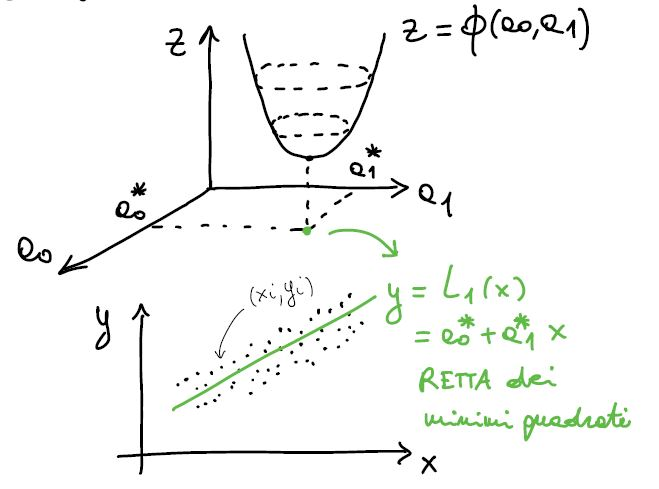
\includegraphics[scale=0.7]{calcolo12.JPG}
\end{center}
Si può anche osservare che definita la matrice di Vandermonde rettangolare
\[
V = (v_{ij}) = (x_i^j)
\]
con $1 \leq i \leq N$ e $0 \leq j \leq m$ cioè\\
\[
V = 
\begin{pmatrix}
1 & x_1 & x_1^2 & \dotso & x_1^m \\
1 & x_2 & x_2^2 & \dotso & x_2^m \\
\vdots & \vdots & \vdots & & \vdots \\
1 & x_N & x_N^2 & \dotso & x_N^m
\end{pmatrix}
\in \mathbb{R}^{N \times (m+1)}
\]
si ha che
\[
\begin{split}
    \phi (a) = \sum_{i=1}^N (y_i - (Va)_i)^2\\
    = (y - Va, y - Va)
\end{split}
\]
dove $(Va)_i$ indica l'elemento i-esimo
del prodotto matrice-vettore
\[
Va = V \cdot 
\begin{pmatrix}
a_0 \\ a_1 \\ \vdots \\ a_m
\end{pmatrix}
= \left \{ \sum_j v_{ij} \cdot a_j \right \} = \left \{ \sum_j x_i^j a_j \right \}
\]
e $(u,v)$ indica il prodotto scalare di due vettori di $\mathbb{R}^N$, cioè 
\[
\begin{split}
(u,v) = \sum\limits_{i=1}^N u_i \cdot v_i \\
(u,u) = \sum\limits_{i=1}^N u_i^2
\end{split}
\]
(quest'ultimo si può interpretare come il quadrato della lunghezza del vettore $u$ che è $\sqrt{(u,u)}$, si pensi a $N=2$ e $N=3$ via teorema di Pitagora).\\
Quindi geometricamente minimizzare $\phi(a)$ significa minimizzare la
lunghezza (o il suo quadrato, che è lo stesso) del vettore $y - Va \in \mathbb{R}^N$ come funzione di $a \in \mathbb{R}^{m+1}$.\\
Enunciamo ora il risultato principale sull'approssimazione polinomiale ai minimi quadrati.

\subsection{TEOREMA (sistema delle equazioni ``normali" per i minimi quadrati)}
\begin{center}
\fbox{\begin{minipage}[t]{0.8\textwidth}
Dati $N$ punti $\{ (x_i, y_i) \}, \ y_i = f(x_i), \ 1 \leq i \leq N$ e $m < N$, il vettore $a \in \mathbb{R}^{m+1}$\\
minimizza $\phi(a) = \sum\limits_{i=1}^N (y_i - \sum\limits_{j=0}^m a_j \cdot x_i^j)^2 \iff $ risolve il sistema $V^t Va = V^t y$. \\
Dove $V^t$ è la trasposta di $V$.
\end{minipage}}
\end{center}
Prima di dimostrare il teorema, osserviamo che il sistema, detto \uline{sistema delle equazioni normali}, ha dimensione $(m+1) \times  (m+1)$: infatti:
\[
	V \in \mathbb{R}^{N \times (m+1)}, \quad V^t \in \mathbb{R}^{(m+1) \times N}, \quad y \in \mathbb{R}^{N}
\]
e quindi:
\[
	V^tV \in \mathbb{R}^{(m+1) \times (m+1)} \text{ e } V^ty \in \mathbb{R}^{m+1}
\]
(qualunque sia il numero di dati: quando si cerca la retta dei minimi quadrati, $m=1$, possono esserci $100, \, 1000, \, 100000$ dati ma il sistema è sempre $2 \times 2$ perchè si cercano $2$ coefficienti).

\subsubsection{\uline{Dimostrazione:}}
\begin{proof}[\unskip\nopunct]
Dire che $a \in \mathbb{R}^{m+1}$ è di minimo (assoluto) per $\phi(a)$ equivale a dire che:
\[
	\phi(a+b) \geq \phi(a) \quad \forall b \in \mathbb{R}^{m+1}
\]
ma
\begin{align*}
    \phi(a+b) & = (y-V(a+b),\, y-V(a+b)) \\
    & = (y-Va-Vb, \, y-Va-Vb) \\
    & = (y-Va,\, y-Va) + (y-Va, \, -Vb) + (-Vb, \, y-Va) + (-Vb, \, -Vb)\\
    & = \phi(a) + 2(Va-y, \, Vb) + (Vb, \, Vb) \\
    & = \phi(a) +2(V^t(Va-y), \, b) + (Vb, \, Vb)
\end{align*}

dove abbiamo usato le seguenti proprietà del prodotto scalare in $\mathbb{R}^{m}$ (per chiarezza indicato con $(u,v)_n$; ricordiamo che $(u,v)_n=u^tv$ interpretando i vettori come vettori-colonna):
\begin{enumerate}
\item $(u,v)_n=(v,u)_n \quad u,v,w \in \mathbb{R}^{n}$
\item $(\alpha u,v)_n= \alpha(u,v)_n \quad \alpha \in \mathbb{R}$
\item $(u+v,w)_n=(u,w)_n+(v,w)_n$
\item $(u,Az)_n = (A^tu,z)_k \quad u \in \mathbb{R}^{n}, \; z \in \mathbb{R}^{k}, \; A \in \mathbb{R}^{n \times k}$
\end{enumerate}
In particolare la 4) è stata usata per scrivere
\[
    \equalto{(Va-y, \, Vb)}{(Va-y, \, Vb)_N} = \equalto{(V^t(Va-y), \, b)}{(V^t(Va-y), \, b)_{m+1}}
\]
\begin{itemize}
\item Dimostriamo per prima l'implicazione ``$\Leftarrow$": assumendo che $V^t Va=V^t y$ abbiamo che:
\[
	V^tVa-V^ty=V^t(Va-y)=0 \quad \text{e} \quad (V^t(Va-y), \, b)=\equalto{(0,b)}{\text{vettore nullo in }\mathbb{R}^{m+1}} =0
\]
da cui:
\[ \begin{split}
	\phi(a+b)=\phi(a)+ \equalto{(Vb,\, Vb)}{\sum_{i=1}^{N}(Vb)_i^2 \geq 0} \geq \phi(a) \quad b \in \mathbb{R}^{m+1}
\end{split} \]
\item Per dimostrare ``$\Rightarrow$", assumiamo che
\[
	\phi(a+b) \geq \phi(a) \quad \forall b \in \mathbb{R}^{m+1}
\]
Allora:
\[ \begin{split}
	\phi(a+b)=\phi(a)+2(V^t(Va-y), \, b)+(Vb,Vb) \geq \phi(a) \quad \forall b
\end{split} \]
Cioè:
\[
	2(V^t(Va-y), \, b) + (Vb,Vb) \geq 0 \quad \forall b
\]
Prendiamo $b=\varepsilon v$, con $v$ versore (cioè vettore di lunghezza 1, $(v,v)=1$). Si ha:
\[ \begin{split}
	& 2(V^t(Va-y), \, \varepsilon v)+(V(\varepsilon v), \, V(\varepsilon v)) = \\
	& = 2\varepsilon (V^t(Va-y), \, v) + \varepsilon^2(Vv,Vv) \geq 0 \quad \forall \varepsilon \geq 0 \text{ e } \forall v
\end{split} \]
Dividendo per $\varepsilon > 0$:
\[ \begin{split}
	2(V^t(Va-y), \, v) + \varepsilon(Vv,Vv) \geq 0 \quad \forall \varepsilon \text{ e } \forall v
\end{split} \]
Per $\varepsilon \to 0$ la disuguaglianza viene mantenuta, ottenendo:
\[ \begin{split}
	(V^t(Va-y), \, v) \geq 0 \quad \forall v
\end{split} \]
Ma se vale $\forall$ versore, possiamo prendere $-v$ al posto di $v$ e otteniamo:
\[ \begin{split}
	(V^t(Va-y), \, -v)=-(V^t(Va-y), \, v) \geq 0 \quad \forall v
\end{split} \]
Cioè $(V^t(Va-y), \, v) \leq 0$, $\forall v$. Siccome $(V^t(Va-y), \, v)$ risulta sia $\geq 0$ che $\leq 0$, allora è $0$:
\[ \begin{split}
	(V^t(Va-y), \, v)=0 \quad \forall v
\end{split} \]
Ma chi è l'unico vettore ortogonale a tutti i vettori? \'E il vettore nullo, cioè
\[ \begin{split}
	V^t(Va-y)=0 \iff V^tVa=V^ty
\end{split} \]
Ovvero $a$ è soluzione del sistema delle equazioni normali.
\end{itemize}
\end{proof}

\subsection{Proprietà di $V^tV$}
A questo punto è importante studiare le proprietà della matrice (quadrata) $V^tV\in\mathbb{R}^{(m+1)\times(m+1)}$.\\Innanzitutto osserviamo che è simmetrica (ricordando che $(AB)^t=B^tA^t$ $\forall A,B$ matrici compatibili per il prodotto), infatti $(V^t V)^t=V^t(V^t)^t=V^tV$. Inoltre $V^tV$ è \uline{semidefinita positiva}, cioè $(V^tVv,v)\geq0$ $\forall v\in\mathbb{R}^{m+1}$.\\ Infatti
\begin{equation*}
    (V^tVv,v)_{m+1}=(Vv,(V^t)^tv)_N=(Vv,Vv)_N\geq0\  \  \  \forall v
\end{equation*}
È noto dall'algebra lineare che allora $V^tV$ ha tutti gli autovalori $\geq0$: ci interessa sapere quando sono tutti $>0$, cioè quando è \uline{definita positiva} (nel qual caso è non singolare, quindi invertibile e il sistema delle equazioni normali ha soluzione unica). Ricordiamo che \uline{definita positiva} significa:
\begin{center}
     $(V^tVv,v)\geq0$ \  \  \   \   $\forall v$   \\
     $(V^tVv,v)=0$  \  \  \  \   solo se $v=0$
\end{center}
Abbiamo appena visto che\\
$(V^tVv,v)=(Vv,Vv)$.\\Ora $(Vv,Vv)=0 \iff Vv=0$ quindi $v=0$ se $V$ ha rango massimo ($rango(V)=m+1$), cioè se le colonne di $V$ sono linearmente indipendenti; ricordiamo che $Vv$ si può interpretare come combinazione lineare delle colonne di $V$ con coefficenti gli elementi di $v$:
\begin{equation*}
    v=(\alpha_1,...,\alpha_{m+1})^t\Rightarrow Vv=\sum_{j=1}^{m+1}\alpha_jC_j(V)
\end{equation*}
Ora è facile dare una condizione che garantisca $rango(V)=m+1$:
basta che ci siano almeno $m+1$ punti distinti tra i nodi di campionamento.\\Supponiamo infatti che siano i primi $m+1$, cioè $x_1,...,x_{m+1}$ con $x_i\neq x_j$, $i\neq j$, $1\leq i$, $j\leq m+1$ (altrimenti basta riordinarli)
\[
    V = 
\begin{pmatrix}
1 & x_1 & x_1^2 & \dotso & x_1^m \\
1 & x_2 & x_2^2 & \dotso & x_2^m \\
\vdots & \vdots & \vdots & & \vdots \\
1 & x_{m+1} & x_{m+1}^2 & \dotso & x_{m+1}^m \\
1 & x_{m+2} & x_{m+2}^2 & \dotso & x_{m+2}^m \\
\vdots & \vdots & \vdots & & \vdots \\
1 & x_N & x_N^2 & \dotso & x_N^m
\end{pmatrix}
\text{Vandermonde di interpolazione = } U \in \mathbb{R}^{(m+1) \times (m+1)}
\]

La sottomatrice $V\in\mathbb{R}^{(m+1)(m+1)}$ nel riquadro è una matrice di Vandermonde\\
per l'interpolazione di grado $\leq m$ su $m+1$ nodi distinti, quindi è non singolare come sappiamo dalla teoria dell'interpolazione (attenzione: qui non stiamo interpolando, il polinomio dei minimi quadrati interpola solo se $m=N-1$, ma tipicamente $m\leq N$; stiamo solo usando una proprietà delle matrici di interpolazione).\\Ma allora il rango della sottomatricd è $m+1$, cioè le sue $m+1$ colonne sono linearmente indipendenti (come vettori di $\mathbb{R}^{m+1}$).\\
Di conseguenza le intere $m+1$ colonne di $V$ sono linearmente indipendenti come vettori di $\mathbb{R}^N$: se fossero linearmente dipendenti, questa proprietà si trasferirebbe alle sottocolonne formate dai primi $m+1$ elementi, infatti se
\[\exists \alpha \ne 0: \sum_{j=1}^{m+1} \alpha_j \, \mathcal{C}_j(V) = 0\]
allora
\[\sum_{j=1}^{m+1} \alpha_j \, \mathcal{C}_j(U) = 0\]
perchè
\[\mathcal{C}_j(V) = 
\begin{pmatrix}
x_1^{j-1}\\ \vdots \\ x_{m+1}^{j-1} \\ x_{m+2}^{j-1} \\ \vdots \\ x_N^{j-1}
\end{pmatrix}
\quad \text{dove} \quad
\begin{pmatrix}
x_1^{j-1}\\ \vdots \\ x_{m+1}^{j-1}
\end{pmatrix}
= \mathcal{C}_j(U)\]
A questo punto possiamo calcolare esplicitamente gli elementi della matrice $V^t V$ (che dipendono solo dagli $\{x_i\}$) e del vettore termine noto $V^ty$ (che dipendono anche dagli $\{y_i\}$)
\[\begin{split}
    V^tV & = \begin{pmatrix}
        1 & 1 & \dotso & \dotso & 1 \\
        x_1 & x_2 & \dotso & \dotso & x_N \\
        \vdots & \vdots & & & \vdots \\
        x_1^m & x_2^m & \dotso & \dotso & x_N^m
    \end{pmatrix} \cdot
    \begin{pmatrix}
        1 & x_1 & \dotso & x_1^m \\
        1 & x_2 & \dotso & x_2^m \\
        \vdots & \vdots & & \vdots \\
        \vdots & \vdots & & \vdots \\
        1 & x_N & \dotso & x_N^m
    \end{pmatrix} \\
    & = \begin{pmatrix}
        N & \sum x_i & \dotso & \sum x_i^m \\
        \sum x_i & \sum x_i^2 & \dotso & \sum x_i^{m+1} \\
        \vdots & \vdots & & \vdots \\
        \sum x_i^m & \sum x_i^{m+1} & \dotso & \sum x_i^{2m}
    \end{pmatrix} \in \mathbb{R}^{(m+1)\times(m+1)}
\end{split}\]
Dove $V^t \in \mathbb{R}^{(m+1)\times N}$ e $V \in \mathbb{R}^{N\times (m+1)}$
\[
V^t y =
\begin{pmatrix}
1 & 1 & \dotso & \dotso & 1 \\
x_1 & x_2 & \dotso & \dotso & x_N \\
\vdots & \vdots & & & \vdots \\
x_1^m & x_2^m & \dotso & \dotso & x_N^m
\end{pmatrix}
\cdot
\begin{pmatrix}
y_1 \\ \vdots \\ \vdots \\ \vdots \\ y_N
\end{pmatrix}
=
\begin{pmatrix}
\sum y_i \\
\sum x_i \cdot y_i \\ \vdots \\ \sum x_i^m \cdot y_i
\end{pmatrix}
\]
Dove $y \in \mathbb{R}^N$ e $V^t \cdot y \in \mathbb{R}^{m+1}$\\
Ad esempio, per $m=1$ (retta dei minimi quadrati) il sistema delle equazioni normali è
\[
\begin{pmatrix}
N & \sum x_i \\
\sum x_i & \sum x_i^2
\end{pmatrix}
\cdot
\begin{pmatrix}
a_0 \\ a_1
\end{pmatrix}
=
\begin{pmatrix}
\sum y_i \\
\sum x_i \cdot y_i
\end{pmatrix}
\]
mentre per $m=2$ (parabola dei minimi quadrati)
\[\begin{pmatrix}
N & \sum x_i & \sum x_i^2 \\
\sum x_i & \sum x_i^2 & \sum x_i^3 \\
\sum x_i^2 & \sum x_i^3 & \sum x_i^4
\end{pmatrix}
\cdot
\begin{pmatrix}
a_0 \\ a_1 \\ a_2
\end{pmatrix}
=
\begin{pmatrix}
\sum y_i \\
\sum x_i \cdot y_i \\
\sum x_i^2 \cdot y_i
\end{pmatrix}\]
Si vede facilmente che la retta dei minimi quadrati ha coefficienti, posto $d = N(\sum x_i^2) - (\sum x_i)^2$
\[
\begin{split}
a_0^* = \frac{1}{d} \cdot ((\sum y_i) \cdot (\sum x_i^2) - (\sum x_i) \cdot (\sum x_i \cdot y_i))\\
a_1^* = \frac{1}{d} \cdot (N \cdot (\sum x_i \cdot y_i) - (\sum x_i) \cdot (\sum y_i)
\end{split}
\]
Per quanto riguarda la soluzione del sistema delle equazioni normali nel caso generale, vedremo nel capitolo dedicato all'algebra lineare numerica che è possibile applicare un metodo (fattorizzazione QR di V) che evita addirittura di calcolare $V^t V$ ed è più stabile del classico metodo di eliminazione gaussiana.\\
Possiamo concludere con qualche cenno sulla scelta del grado $m$ per il polinomio $L_m$ dei minimi quadrati. Tipicamente, come abbiamo detto, si prende $m<<N$, con scelta che può essere suggerita, almeno qualitativamente, dall'aspetto grafico dei dati e quantitativamente dalla grandezza di $min\  \phi(a)$ al variare di $m$, oppure dall'errore di approssimazione di alcuni dati campionati $\{(\tilde{x_j},\tilde{y_j})\}$ che non si usano nella costruzione ma
si tengono per controllo calcolando ad esempio $max_j\  |\tilde{y_j}-L_m(\tilde{x_j})|$.\\Per chiarire, tornando all'esempio iniziale di un segnale con rumore
\begin{center}
    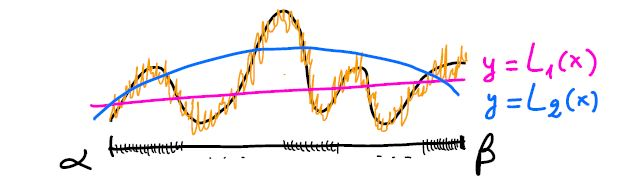
\includegraphics[scale=0.7]{calcolo32.JPG}
\end{center}
è chiaro che le approssimazioni con $m=1$ e $m=2$ sono del tutto inadeguate per ricostruire il segnale (che ha 5 estremi locali interni), per cui ci si aspetta che possa essere efficace solo un opportuno grado $m>6$.\\
Non ci addentriamo nella difficile questione teorica di quali siano possibili distribuzioni di nodi (con $N$ dipendente da $m$) che garantiscono la convergenza 
\[
dist(f, L_m) \to 0, \ m \to \infty
\]
per $f \in C^k[\alpha, \beta]$.\\
(nota facoltativa: si può ad esempio dimostrare, ma la dimostrazione è difficile e richiede nozioni avanzate di teoria dell'approssimazione polinomiale, che $N = c \cdot m^2$ nodi equispaziati con $c>1$ vanno bene per $k>1$ nel senso che $\exists c_k > 0$ tale che $dist(f,L_m) \leq c_k \cdot m^{1-k}$).

\end{document}